% Copyright (c) 2026 Islam Ibrahim. All rights reserved.

\documentclass[tikz,border=8pt]{standalone}
\usepackage[T1]{fontenc}
\usepackage{lmodern}
\usepackage{amsmath}
\usepackage{tikz}
\usetikzlibrary{arrows.meta,decorations.pathmorphing,positioning}

\begin{document}
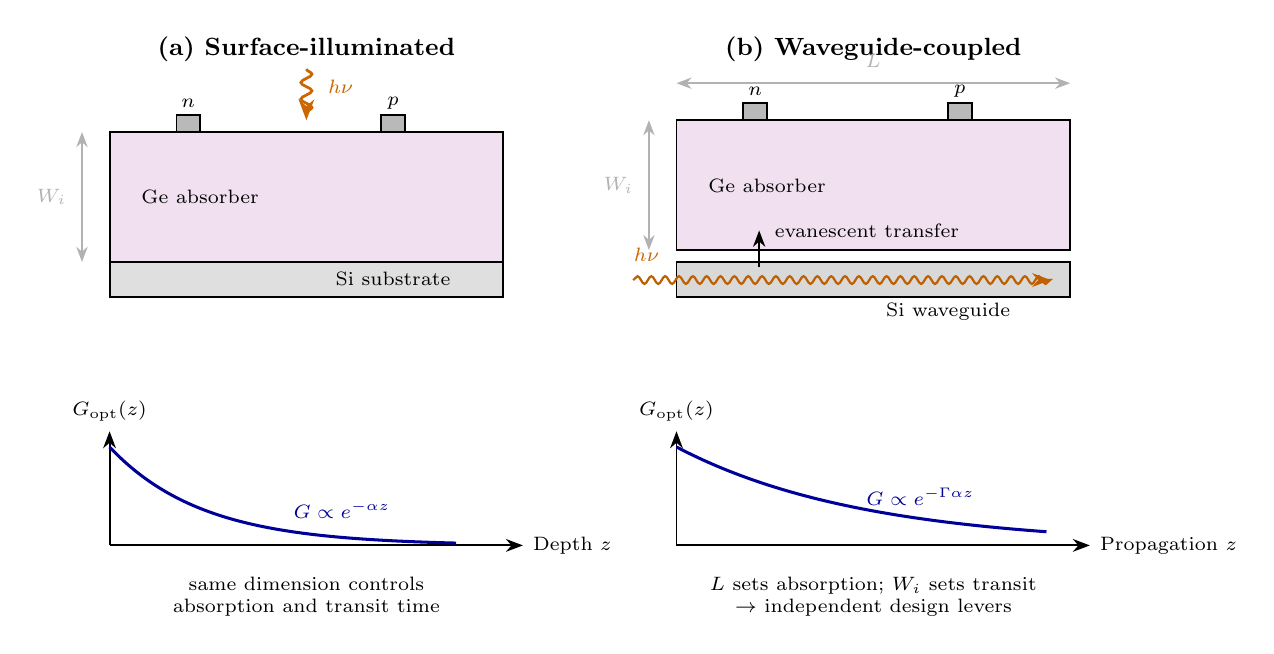
\begin{tikzpicture}[font=\small\rmfamily,>=Stealth,
  lbl/.style={font=\scriptsize\rmfamily},
  ax/.style={line width=0.7pt,->},
  seg/.style={line width=1.1pt,black},
  box/.style={draw=black,line width=0.7pt},
]

\def\W{5.0}
\def\H{1.65}
\def\subH{0.45}
\def\plotY{-2.05}
\def\xsep{7.2}

% ------------------------------------------------------------------
% Panel A: surface illuminated
% ------------------------------------------------------------------
\begin{scope}
  \node[font=\small\bfseries\rmfamily] at (\W/2,4.25)
    {(a) Surface-illuminated};

  \fill[violet!12,box] (0,1.55) rectangle (\W,1.55+\H);
  \node[lbl] at (1.15,2.38) {Ge absorber};
  \fill[gray!25,box] (0,1.10) rectangle (\W,1.55);
  \node[lbl] at (3.60,1.33) {Si substrate};

  \fill[gray!55,box] (0.85,3.20) rectangle (1.15,3.42);
  \fill[gray!55,box] (3.45,3.20) rectangle (3.75,3.42);
  \node[lbl] at (1.00,3.57) {$n$};
  \node[lbl] at (3.60,3.57) {$p$};

  \draw[line width=1.0pt,orange!80!black,
    decorate,decoration={snake,amplitude=2pt,segment length=6pt},->]
    (2.50,4.00) -- (2.50,3.35);
  \node[lbl,orange!80!black,right=2pt] at (2.58,3.78) {$h\nu$};

  \draw[<->,line width=0.55pt,gray!60]
    (-0.35,1.55) -- (-0.35,3.20)
    node[midway,left=2pt,lbl,gray!60]{$W_i$};

  \draw[ax] (0,\plotY) -- (\W+0.25,\plotY) node[right,lbl]{Depth $z$};
  \draw[ax] (0,\plotY) -- (0,\plotY+1.45) node[above,lbl]{$G_\mathrm{opt}(z)$};
  \draw[seg,blue!60!black,domain=0.0:4.4,samples=80,variable=\t]
    plot (\t, {\plotY+1.25*exp(-0.85*\t)});
  \node[lbl,blue!60!black] at (2.95,\plotY+0.45) {$G\propto e^{-\alpha z}$};

  \node[lbl,align=center] at (\W/2,\plotY-0.65)
    {same dimension controls\\absorption and transit time};
\end{scope}

% ------------------------------------------------------------------
% Panel B: waveguide integrated
% ------------------------------------------------------------------
\begin{scope}[xshift=\xsep cm]
  \node[font=\small\bfseries\rmfamily] at (\W/2,4.25)
    {(b) Waveguide-coupled};

  \fill[violet!12,box] (0,1.70) rectangle (\W,1.70+\H);
  \node[lbl] at (1.15,2.52) {Ge absorber};
  \fill[gray!30,box] (0,1.10) rectangle (\W,1.55);
  \node[lbl] at (3.45,0.92) {Si waveguide};

  \fill[gray!55,box] (0.85,3.35) rectangle (1.15,3.57);
  \fill[gray!55,box] (3.45,3.35) rectangle (3.75,3.57);
  \node[lbl] at (1.00,3.72) {$n$};
  \node[lbl] at (3.60,3.72) {$p$};

  \draw[line width=0.8pt,orange!75!black,
    decorate,decoration={snake,amplitude=1.4pt,segment length=5pt},->]
    (-0.55,1.32) -- (4.75,1.32);
  \node[lbl,orange!80!black,above=3pt] at (-0.38,1.32) {$h\nu$};

  \draw[line width=0.65pt,->] (1.05,1.48) -- (1.05,1.95)
    node[right=2pt,lbl]{evanescent transfer};

  \draw[<->,line width=0.55pt,gray!60]
    (-0.35,1.70) -- (-0.35,3.35)
    node[midway,left=2pt,lbl,gray!60]{$W_i$};
  \draw[<->,line width=0.55pt,gray!60]
    (0,3.82) -- (\W,3.82)
    node[midway,above=2pt,lbl,gray!60]{$L$};

  \draw[ax] (0,\plotY) -- (\W+0.25,\plotY) node[right,lbl]{Propagation $z$};
  \draw[ax] (0,\plotY) -- (0,\plotY+1.45) node[above,lbl]{$G_\mathrm{opt}(z)$};
  \draw[seg,blue!60!black,domain=0.0:4.7,samples=90,variable=\t]
    plot (\t, {\plotY+1.25*exp(-0.42*\t)});
  \node[lbl,blue!60!black] at (3.10,\plotY+0.62) {$G\propto e^{-\Gamma\alpha z}$};

  \node[lbl,align=center] at (\W/2,\plotY-0.65)
    {$L$ sets absorption; $W_i$ sets transit\\$\rightarrow$ independent design levers};
\end{scope}

\end{tikzpicture}
\end{document}
